\section{Relationship with the architecture}
%This section should list the inconsistencies between your architecture and the implementation. Give the reasons for these inconsistencies. Discuss whether they could have been discovered at an earlier point, for instance during the ATAM evaluation.

Although we initially planned to only have views on the client. and keep all controllers and models on the server, we found it necessary to have network-controllers and local replica models client side as well, and as you can see our final class diagram in figure \ref{fig:class_diagram_server}, is structured a bit differently from the original, which can be seen in figure \ref{fig:old-class-diagram}. One cal also notice that filenames are different from what we planned.

However, we realized this early in the process, just after we had handed in the architectural report and before we started started writing any code, so even if we have discovered it earlier, it wouldn't have made a significant difference. It was not really mentioned in the ATAM evaluation, as we gave notice to our evaluation team that we probably would have to do something like that.

\begin{figure}[H]
    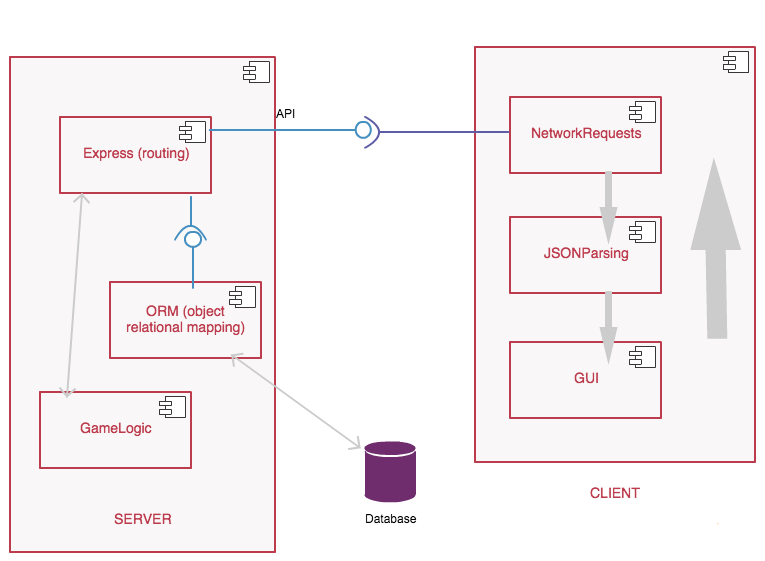
\includegraphics[scale=0.5]{figs/component.png}
    \caption{Our component diagram form the architectural documentation.}
    \label{fig:old-component-diagram}
\end{figure}

\begin{figure}[H]
    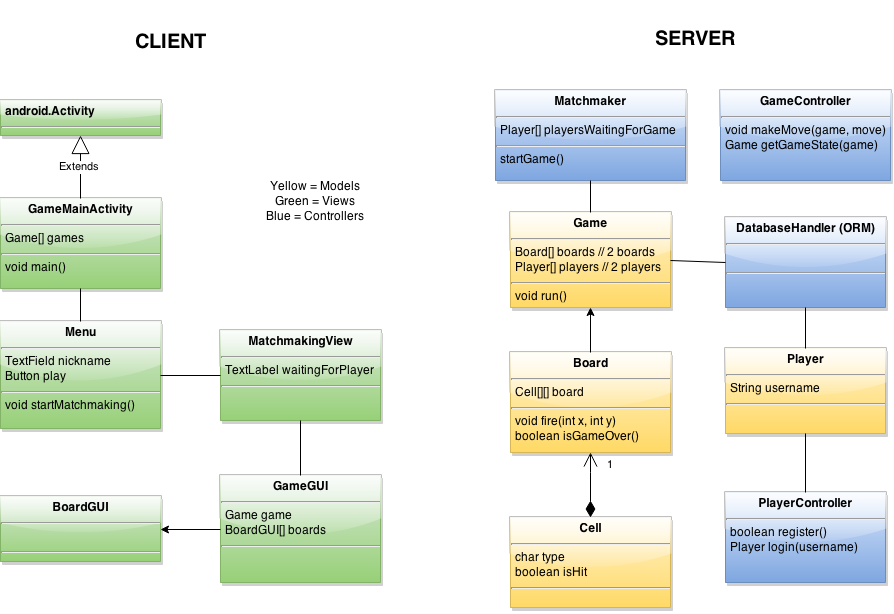
\includegraphics[scale=0.5]{figs/old-class-diagram.png}
    \caption{The class diagram from the architectural documentation. }
    \label{fig:old-class-diagram}
\end{figure}

One can also notice the inconsistencies between the final class diagrams on the client, and the planned component diagram in figure \ref{fig:old-component-diagram}, especially when it comes to data flow. Where we originally thought that the component handling the network requests would be a simple entity only communicating with a JSON-component, we that in practice this became a lot more complicated. The models are the ones that uses JSON-parser for the most part, and we had to make two controllers to handle the network requests, which also has to handle some view- and model-related tasks.

We could have made a more detailed plan for the the network logic, models and the relationship to the GUI more detailed. JAVA is an object-oriented language, and one needs to think in terms of objects all the time, so it makes sense to have Board, Cell and Player models. 

On the server, we planned to have a Cell object, but this was an unnecessary complication. A cell is only a char in a board string in the database, and we just create a simple cell with two booleans when we want it. This is done directly in the JSON data object that is to be sent to the client. 


